\section{Training Neural Networks}\label{sec:train-nn}

\subsection{Activation Functions}\label{sec:tnn-activation}

In section \ref{dl-activation} we introduced some activation functions. Now we are going to dive into deeper details to point out which is better to use.

\begin{figure}[h!]
    \centering
    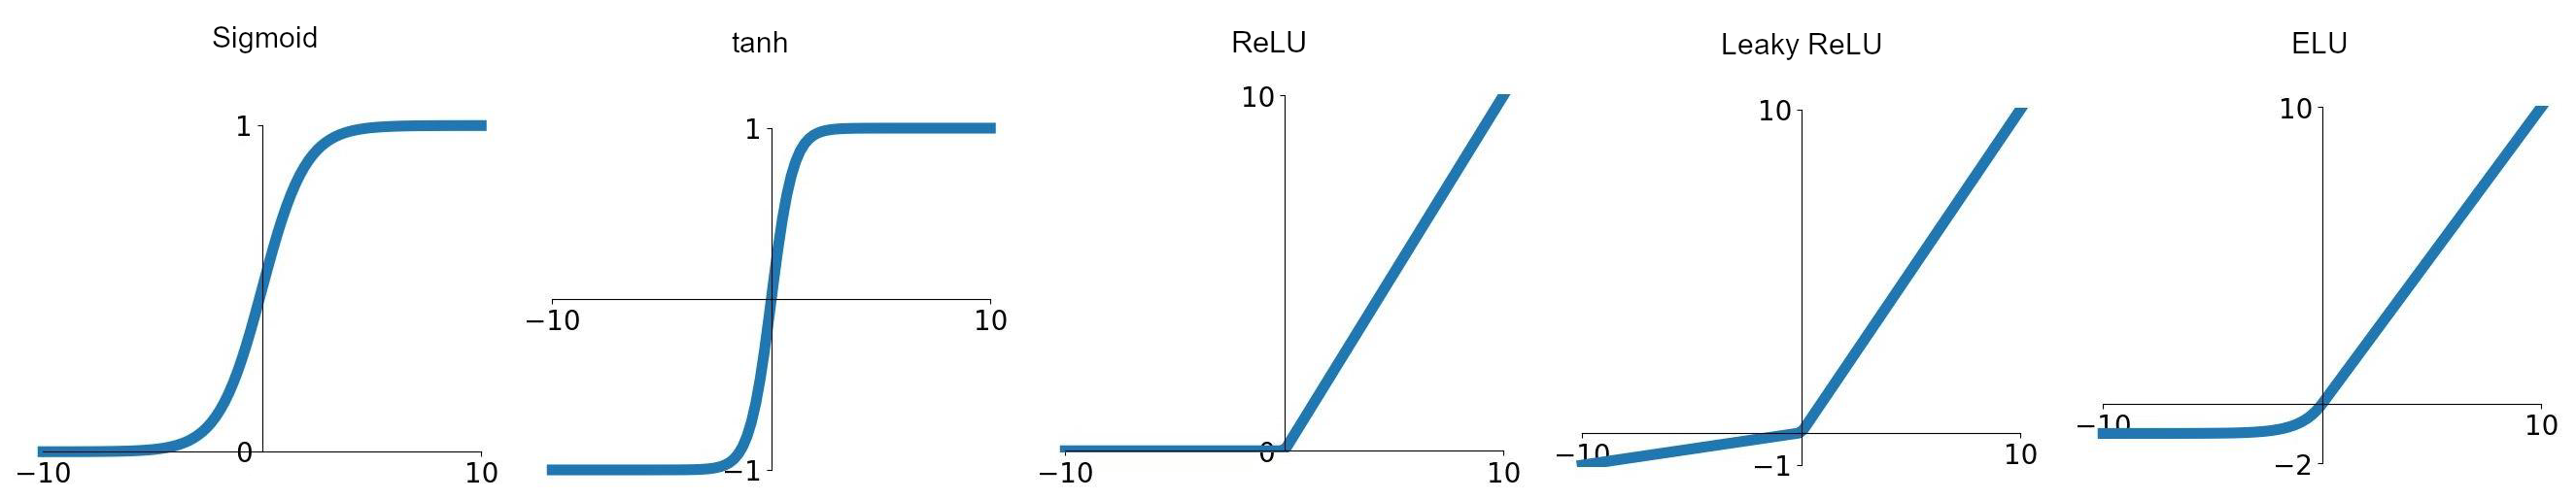
\includegraphics[width=\linewidth]{activations}
    \caption[Some activation functions]{Some activation functions}
    \label{fig:activations}
\end{figure}

\begin{myitem}
    \item \textbf{Sigmoid} $\sigma(x) = \frac{1}{1 + e^{-x}}$:
    \begin{itemize}
        \item squashes numbers to range $[0,1]$;
        \item historically popular since they have nice interpretation as a saturating “firing rate” of a neuron;
        \item problems: saturated neurons kill the gradients, outputs are not zero-centered, \texttt{exp()} is a bit computationally expensive;
        \item if the input of a neuron is always positive, the gradients of the relative weights are all positive or all negative.
    \end{itemize}
    \item \textbf{Tanh} $\tanh(x)$:
    \begin{itemize}
        \item squashes numbers to range $[-1,1]$;
        \item outputs \textit{are} zero-centered;
        \item problem: saturated neurons kill the gradients.
    \end{itemize}
    \item \textbf{ReLU} $\max(0,x)$:
    \begin{itemize}
        \item does not saturate in positive region;
        \item very computationally efficient;
        \item converges much faster than \textit{sigmoid} or \textit{tanh};
        \item problems: outputs are not zero-centered, if the input is negative the dead \textit{ReLU} will never activate and never update weights;
        \item people like to initialize \textit{ReLU} neurons with slightly positive biases.
    \end{itemize}
    \item \textbf{Leaky ReLu} $\max(0.1x,x)$:
    \begin{itemize}
        \item has all the advantages of \textit{ReLU};
        \item does not ``die''.
    \end{itemize}
    \item \textbf{Parametric Rectifier - PReLU} $\max(\alpha x, x)$:
    \begin{itemize}
        \item similar to \textit{Leaky ReLU};
        \item backpropagation into $\alpha$ parameter.
    \end{itemize}
    \item \textbf{Exponential Linear Units - ELU}
    $\begin{cases}
    x              &x \geq 0\\
    \alpha(e^x -1) &x < 0
    \end{cases}$:
    \begin{itemize}
        \item all benefits of \textit{ReLU};
        \item closer to zero mean outputs;
        \item negative saturation regime compared with \textit{Leaky ReLU} adds some robustness to noise;
        \item problem: \texttt{exp()} is a bit computationally expensive.
    \end{itemize}
    \item \textbf{Maxout ``neuron''}: $\max(W_1^T x + b_1, W_2^T x + b_2)$,
    \begin{itemize}
        \item it is a neuron without the form of dot product (non-linearity);
        \item generalizes \textit{ReLU} and \textit{Leaky ReLU};
        \item advantages: linear regime, does not saturate, does not die;
        \item problem: doubles the number of parameters.
    \end{itemize}
\end{myitem}

To sum up:
\begin{myitem}
    \item Use \textit{ReLU}. Be careful with your learning rates.
    \item Try out \textit{Leaky ReLU}/\textit{Maxout}/\textit{ELU}.
    \item Try out \textit{tanh} but don’t expect much.
    \item Don’t use \textit{sigmoid}.
\end{myitem}


\subsection{Data Preprocessing}\label{sec:tnn-preprocessing}

Possible preprocessing approaches are zero-centering, normalization, PCA (Principle Component Analysis), whitening.

After normalization, classification loss is less sensitive to small changes in weights and easier to optimize.

When dealing with images, it is better to apply only centering, while PCA or whitening aren't common:
\begin{myitem}
    \item subtract the mean image;
    \item subtract per-channel mean;
    \item subtract per-channel mean and divide by per-channel std.
\end{myitem}


\subsection{Weight Initialization}\label{sec:tnn-weights}

In some cases, it is important to carefully initialize weights to avoid saturating the activation:
\begin{myitem}
    \item Small random numbers (\textbf{activation statistics}):
    \begin{itemize}
        \item uses a gaussian with zero mean and 1e-2 standard deviation,
        \item works quite well for small networks,
        \item all activations tend to zero for deeper network layers, so there is no learning, even with a larger std;
    \end{itemize}
    \item \textbf{Xavier initialization}:
    \begin{itemize}
        \item uses std $= \frac{1}{\sqrt{Din}}$, where for convolutional layers $Din = \text{kernel\_size}^2 \cdot \text{input\_channels}$,
        \item assumes zero-centered activation function, thus it doesn't work with ReLU;
    \end{itemize}
    \item \textbf{Kaiming/MSRA initialization}:
    \begin{itemize}
        \item uses std $= \sqrt{\frac{2}{Din}}$,
        \item activations are nicely scaled for all layers.
    \end{itemize}
\end{myitem}

It's worth noting that proper initialization is an active area of research.


\subsection{Batch Normalization}\label{sec:tnn-normalization}

Consider a batch of activations at some layer. To make each dimension zero-mean unit-variance, apply the following formula:
\begin{equation}\label{eq:tnn-normalization-1}
    \hat{x}_{i,j} = \frac{x_{i,j} - \mu_j}{\sqrt{\sigma_j^2 + \varepsilon}}
\end{equation}
where the input $x$ has shape $N \times D$, $\mu_j = \frac1N \sum_{i=1}^{N} x_{i,j}$ (per-channel mean with shape $D$) and $\sigma_j^2 = \frac1N \sum_{i=1}^{N} (x_{i,j} - \mu_j)^2$ (per-channel variance, with shape $D$). The normalized $x$ has shape $N \times D$ too.

If zero-mean and unit-variance is a too hard constraint, we can use a slight different approach:
\begin{equation}\label{eq:tnn-normalization-2}
    y_{i,j} = \gamma_j \hat{x}_{i,j} + \beta_j
\end{equation}
where $\beta$ and $\gamma$ are learnable scale and shift parameters with shape $D$.

Since estimates depend on minibatch, this method can't be used at test time. During testing batch normalization becomes a linear operator, and can be fused with the previous fully connected or convolutional layer.

The Batch Normalization Layer is usually inserted after Fully Connected or Convolutional layers, and before nonlinearity.

Advantages of batch normalization:
\begin{myitem}
    \item Makes deep networks much easier to train;
    \item Improves gradient flow;
    \item Allows higher learning rates, faster convergence;
    \item Networks become more robust to initialization;
    \item Acts as regularization during training;
    \item Zero overhead at test time (since it can be fused with the previous layer).
\end{myitem}

Problem: behaves differently during training and testing, and this is a very common source of bugs.\\
\textbf{Layer Normalization} gives same behavior to at train and test to fully-connected networks, while \textbf{Instance Normalization} does the same job for convolutional networks.

\begin{figure}[h!]
    \centering
    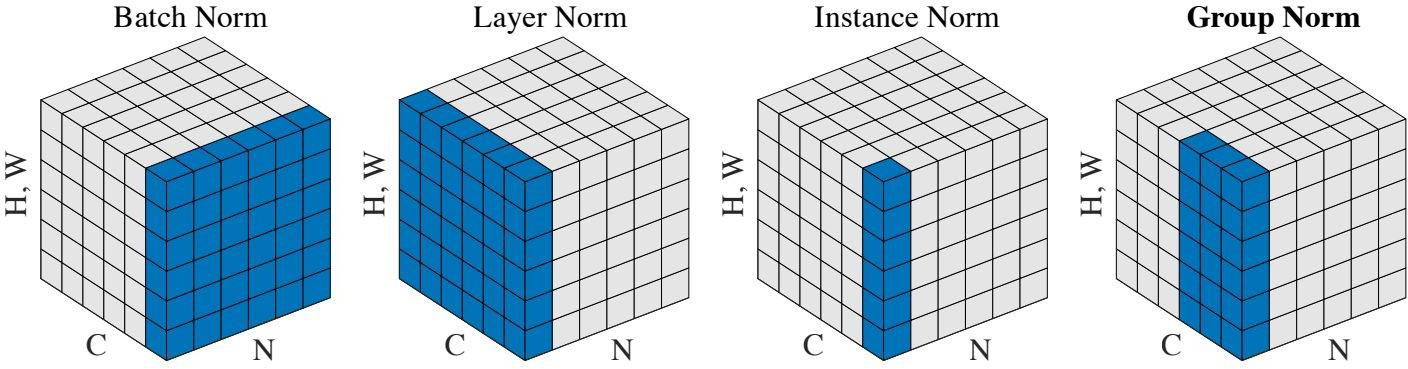
\includegraphics[width=0.7\linewidth]{images/normalization}
    \caption[Normalization types]{Normalization types}
    \label{fig:normalization}
\end{figure}


\subsection{Optimizers}\label{sec:tnn-optimizers}

Stochastic Gradient Descent (introduced in section \ref{bif-sgd}) may present some problems:
\begin{myitem}
    \item If loss changes quickly in one direction and slowly in another, gradient descent progresses slowly along the shallow dimension and jitters along the steep direction. Loss function has high condition number: ratio of largest to smallest singular value of the Hessian matrix is large.
    \item If the loss function has local minima or saddle points, the gradient is zero, thus the gradient descent gets stuck.
    \item Gradients come from mini-batches, so they can be noisy.
\end{myitem}

A possible solution is to add \textbf{Momentum} to the computed gradient: at each iteration the gradient is added to the \textit{velocity} (computed as a running mean of gradients) multiplied by a \textit{friction} factor (typically $\rho = 0.9$ or $0.99$). That is, weights are updated as follows:
\begin{flalign}\label{eq:momentum-1}
    v_{t+1} &= \rho v_t + \nabla f(x_t)\\
    x_{t+1} &= x_t - \alpha v_{t+1}
\end{flalign}

Another possible and equivalent formulation is the following:
\begin{flalign}\label{eq:momentum-2}
    v_{t+1} &= \rho v_t - \alpha \nabla f(x_t)\\
    x_{t+1} &= x_t + v_{t+1}
\end{flalign}

Another option is to use \textbf{Nesterov Momentum}: ``Look ahead'' to the point where updating using velocity would take us, then compute gradient there and mix it with velocity to get actual update direction:
\begin{flalign}\label{eq:momentum-nesterov-1}
    v_{t+1} &= \rho v_t - \alpha \nabla f(x_t + \rho v_t)\\
    x_{t+1} &= x_t + v_{t+1}
\end{flalign}
or, to obtain the update in terms of $f_x$, let be $\tilde{x}_t = x_t + \rho v_t$:
\begin{flalign}\label{eq:momentum-nesterov-2}
    v_{t+1} &= \rho v_t - \alpha \nabla f(\tilde{x}_t)\\
    \tilde{x}_{t+1} &= \tilde{x}_t - \rho v_t + (1- \rho) v_{t+1} \notag\\
    &= \tilde{x}_t + v_{t+1} + \rho (v_{t+1} - v_t)
\end{flalign}

\textbf{AdaGrad} adds element wise scaling of the gradient based on the historical sum of squares in each dimension (\textit{Per parameter learning rates} or \textit{adaptive learning rates}):
\begin{flalign}\label{eq:adagrad}
    gs_{t+1} &= gs_t + (\nabla f(x_{t}))^2\\
    x_{t+1} &= x_t - \alpha \cdot \frac{\nabla f(x_{t})}{\sqrt{gs_{t+1}} + \text{1e-7}}
\end{flalign}
In this way, progress along steep directions is damped, while progress along flat directions is accelerated. Over long time, the step size decays to zero.

With \textbf{RMSProp}, a sort of ``Leaky AdaGrad'', grad squared becomes
\begin{flalign}\label{eq:rmsprop}
    gs_{t+1} &= \text{decay\_rate} \cdot gs_t + (1 - \text{decay\_rate}) \cdot (\nabla f(x_{t}))^2\\
    x_{t+1} &= x_t - \alpha \cdot \frac{\nabla f(x_{t})}{\sqrt{gs_{t+1}} + \text{1e-7}}
\end{flalign}
This solves the problem of radically diminishing learning rates.

\textbf{Adam} optimizer uses first and second moments, plus bias correction for the fact that first and second moment estimates start at zero:
\begin{flalign}\label{eq:adam}
    \text{first\_moment}_{t+1} &=
    \beta_1 \cdot \text{first\_moment}_t + (1 - \beta_1) \cdot \nabla f(x_{t})\\
    \text{second\_moment}_{t+1} &=
    \beta_2 \cdot \text{second\_moment}_t + (1 - \beta_2) \cdot (\nabla f(x_{t}))^2\\
    \text{first\_unbias}_{t+1} &= \frac{\text{first\_moment}_{t+1}}{1 - \beta_1^t}\\
    \text{second\_unbias}_{t+1} &= \frac{\text{second\_moment}_{t+1}}{1 - \beta_2^t}\\
    x_{t+1} &=
    x_t - \alpha \cdot \frac{\text{first\_unbias}_{t+1}}{\sqrt{\text{second\_unbias}_{t+1}} + \text{1e-7}}
\end{flalign}
Adam with $\beta_1 = 0.9, \beta_2 = 0.999$, and learning\_rate = 1e-3 or 5e-4 is a great starting point for many models.

Adaptive learning rates are preferable for faster optimizations, especially as gradients become sparser. \textit{Adam} is the most used.

\begin{minipage}{.5\linewidth}
    \begin{figure}[H]
        \centering
        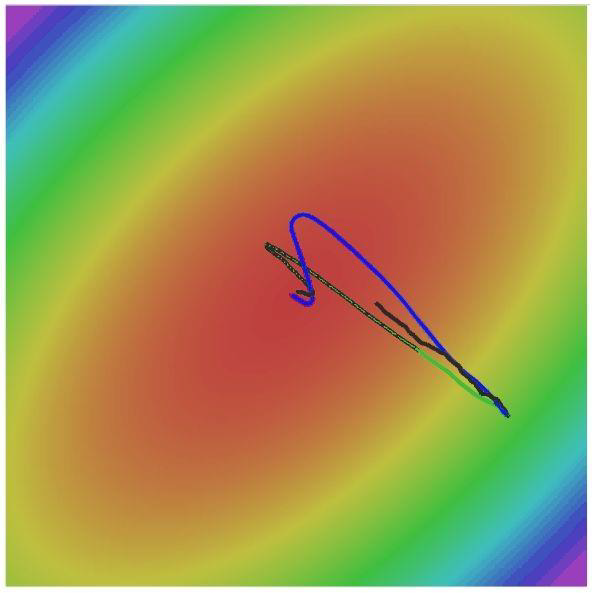
\includegraphics[width=.9\linewidth]{images/momentum}
        \caption[Different kinds of SGD and momentum]{Different kinds of SGD and momentum.\\
            SGD in black, SGD + Momentum in blue,\\Nesterov Momentum in green.}
        \label{fig:momentum-1}
    \end{figure}
\end{minipage}
\begin{minipage}{.5\linewidth}
    \begin{figure}[H]
        \centering
        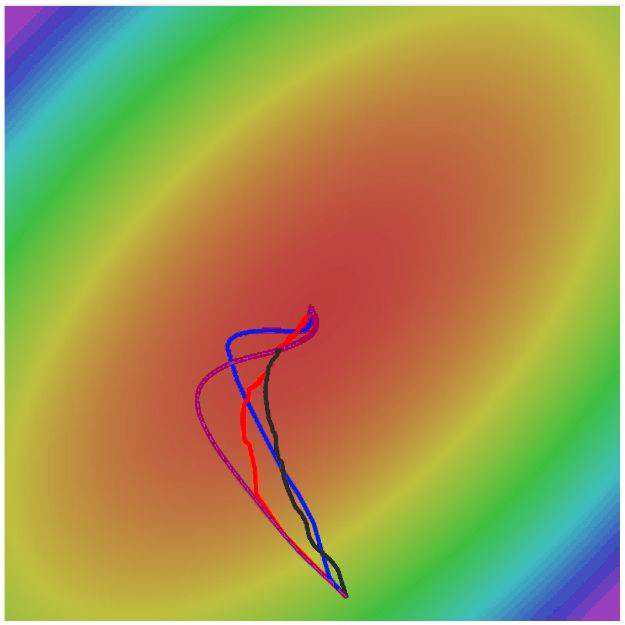
\includegraphics[width=.9\linewidth]{images/momentum1}
        \caption[Different kinds of SGD and optimizers]{Different kinds of SGD and optimizers.\\
            SGD in black, SGD + Momentum in blue, RMSProp in red, Adam in purple.}
        \label{fig:momentum-2}
    \end{figure}
\end{minipage}


\subsection{Learning Rate Decay}\label{sec:tnn-learning-rate}

\textit{SGD}, \textit{SGD+Momentum}, \textit{Adagrad}, \textit{RMSProp}, \textit{Adam} all have learning rate as a hyperparameter, so we have to choose it. It is a good practice to begin with a large learning rate, and decay over time. There are several approaches to learning rate decay; let be $\alpha_0$ the initial learning rate, $\alpha_t$ the learning rate at epoch $t$, $T$ the total number of epochs, then:
\begin{myitem}
    \item \textbf{Step}: reduce learning rate at a few fixed points;
    \item \textbf{Cosine}: $\alpha_t = \frac12 \alpha_0 (1 + \cos(\frac{t \pi}{T}))$;
    \item \textbf{Linear}: $\alpha_t = \alpha_0 (1 - \frac{t}{T})$;
    \item \textbf{Inverse sqrt}: $\alpha_t = \frac{\alpha_0}{\sqrt{t}}$.
\end{myitem}

\textbf{Linear Warmup}: High initial learning rates can make loss explode, linearly increasing learning rate from 0 over the first 5000 iterations can prevent this.

\begin{figure}[h!]
    \centering
    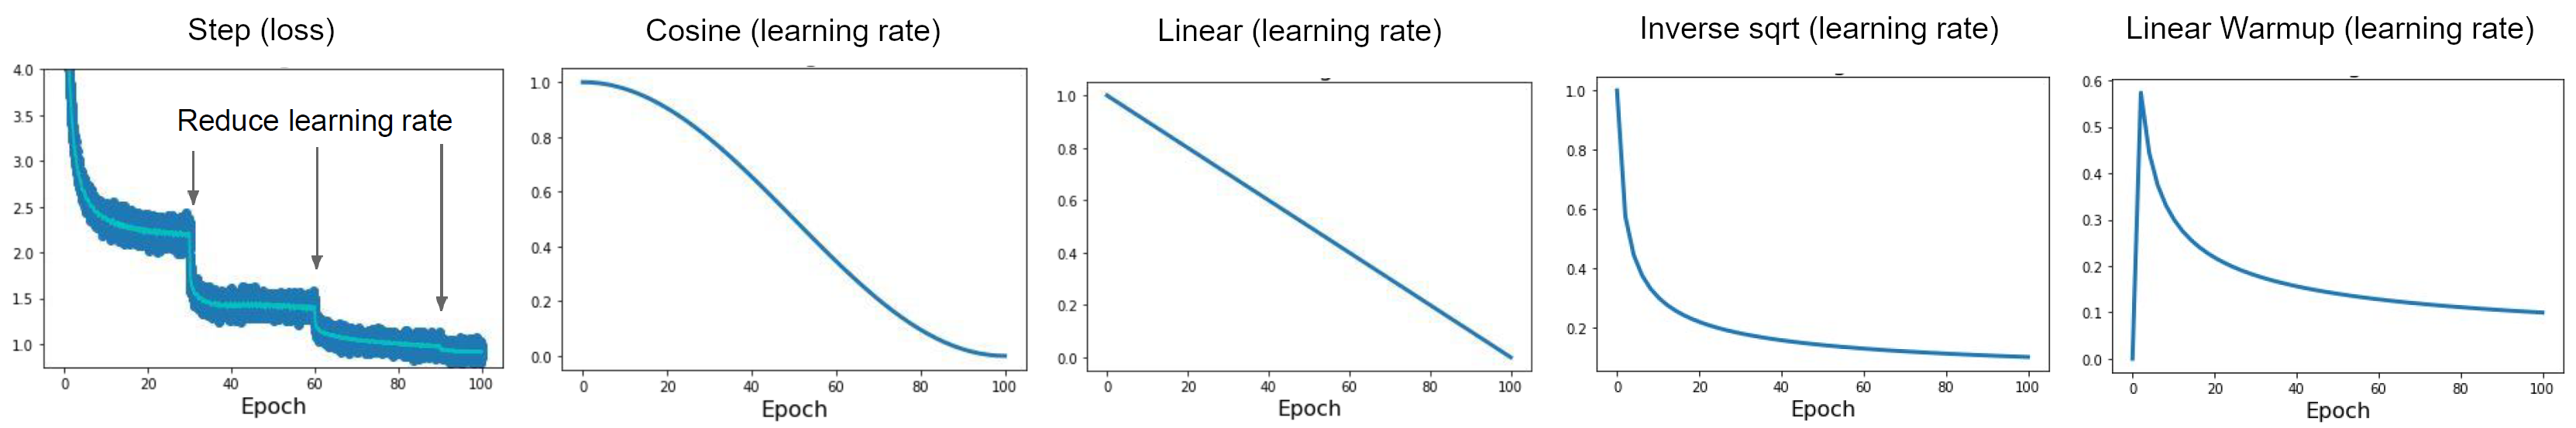
\includegraphics[width=\linewidth]{images/learning-rate}
    \caption[Learning rate decay methods]{Learning rate decay methods}
    \label{fig:learning-rate}
\end{figure}

Empirical rule of thumb: If you increase the batch size by $N$, also scale the initial learning rate by $N$.

In practice, \textit{Adam} is a good default choice in many cases, even with constant learning rate. \textit{SGD+Momentum} can outperform \textit{Adam} but may require more tuning of LR and schedule (try cosine schedule).

Better optimization algorithms help reduce training loss, but we are interested in error on new data. A good way to reduce the gap between the two curves, is to stop training the model when accuracy on the validation set decreases (\textbf{early stopping}).

\textbf{Model Ensembles}:
\begin{myitem}
    \item Train multiple independent models and, at test time, average their results.
    \item Or use multiple snapshots of a single model during training.
    \item Instead of using actual parameter vector, keep a moving average of the parameter vector and use that at test time (\textit{Polyak averaging}).
\end{myitem}


\subsection{Regularization}\label{sec:tnn-regularization}

A common approach to improve single-model performance is to add a term to the loss, such as \textit{L1} or \textit{L2 regularization} or \textit{Elastic net}, as we saw in section \ref{ic-regularization}.

Another possibility is \textbf{Dropout}: in each forward pass, randomly set some neurons to zero, with probability $p$, a hyperparameter. This is useful because it forces the network to have a redundant representation, and prevents co-adaptation of features. Another interpretation: dropout is training a large ensemble of models (that share parameters), where each binary mask is one model.
Because of how it works, dropout makes the output random. At test time we want to average out the randomness:
\begin{equation}\label{eq:dropout-1}
    y = f(x) = E_z[f(x,z)] = \int p(z) f(x,z) dz
\end{equation}
where $y$ is the label, $x$ is the input image, and $z$ is the random mask.\\
The integral can be approximated by multiplying by dropout probability. Consider a single neuron: at test time we have
\begin{equation}\label{eq:dropout-2}
    E[a] = w_1 x + w_2 y,
\end{equation}
during training we have
\begin{flalign}\label{eq:dropout-3}
    E[a] &= \frac14 (w_1 x + w_2 y) + \frac14 (w_1 x + 0 y) +
            \frac14 (0 x + 0 y) + \frac14 (0 x + w_2 y) \notag\\
         &= \frac12 (w_1 x + w_2 y).
\end{flalign}
In other words, at test time all neurons are active always, thus we must scale the activations so that for each neuron \texttt{output at test time = expected output at training time}.

A common pattern for regularization is to add some kind of randomness at training time, and average out that randomness (eventually with some approximation) at testing time. For example, in batch normalization, during training we normalize using statistics from random minibatches, but during testing we use fixed stats to normalize.

Another mechanism which can be used for regularization purposes, is \textbf{Data Augmentation}, obtained through image transformations such as:
\begin{myitem}
    \item \textit{Horizontal flips};
    \item During training sample \textit{random crops and scales}, during test average a fixed set of crops;
    \item \textit{Color jitter}:
    \begin{itemize}
        \item  Randomize contrast and brightness, or
        \item apply PCA to all pixels in training set, sample a ``color offset'' along principal component directions, add offset to all pixels of a training image;
    \end{itemize}
    \item Combination of \textit{translation, rotation, stretching, shearing, lens distortions}...
\end{myitem}

\newpage
Other useful regularization techniques are:
\begin{myitem}
    \item \textbf{DropConnect} drops connections between neurons (setting weights to 0) during training, and uses all the connections in testing;
    \item \textbf{Fractional Pooling} uses randomized pooling regions in training, and average predictions from several regions in testing;
    \item \textbf{Stochastic Depth} skips some layers in the network during training, and uses all the layers in testing;
    \item \textbf{Cutout} sets random image regions to zero during training, and uses full image in testing;
    \item \textbf{Mixup} trains on random blends of images, and tests with original images.
\end{myitem}

In conclusion:
\begin{myitem}
    \item Consider dropout for large
    fully connected layers;
    \item Batch normalization and data augmentation almost always a good idea;
    \item Try cutout and mixup especially for small classification datasets.
\end{myitem}


\subsection{Choosing Hyperparameters}\label{sec:tnn-hyperparameters}

To choose hyperparameters could require a lot of time or computational resources, so it is important to follow a set of guidelines:
\begin{myenum}
    \item \textbf{Check initial loss}: Turn off weight decay, sanity check loss at initialization.
    \item \textbf{Overfit a small sample}: Try to train to 100\% training accuracy on a small sample of training data; fiddle with architecture, learning rate, weight initialization.
    \item \textbf{Find LR that makes loss go down}: Use the architecture from the previous step, use all training data, turn on small weight decay, find a learning rate that makes the loss drop significantly within ~100 iterations.
    \item \textbf{Coarse grid, train for ~1 5 epochs}: Choose a few values of learning rate and weight decay around what worked from Step 3, train a few models for ~1-5 epochs.
    \item \textbf{Refine grid, train longer}: Pick best models from Step 4, train them for longer without learning rate decay.
    \item \textbf{Look at learning curves}:
    \begin{itemize}
        \item Losses may be noisy, use a scatter plot and also plot moving average to see trends better, while plotting \textit{training loss};
        \item In presence of a loss drop, the problem may be bad initialization (see figure \ref{fig:tnn-loss-1});
        \item In case of loss plateaus, try learning rate decay (see figure \ref{fig:tnn-loss-2});
        \item With learning rate step decay, loss was still going down when learning rate dropped, so the decay was too early (see figure \ref{fig:tnn-loss-3});
        \item If \textit{validation accuracy} is still going up, you need to train longer (see figure \ref{fig:tnn-acc-1});
        \item If there is a huge gap between train and validation accuracy, there is overfitting, so increase regularization, or get more data (see figure \ref{fig:tnn-acc-2});
        \item No gap between train/val means underfitting, so train longer, or use a bigger model (see figure \ref{fig:tnn-acc-3}).
    \end{itemize}
    \item \textbf{GOTO step 5}.
\end{myenum}

\begin{minipage}{.3\linewidth}
    \begin{figure}[H]
        \centering
        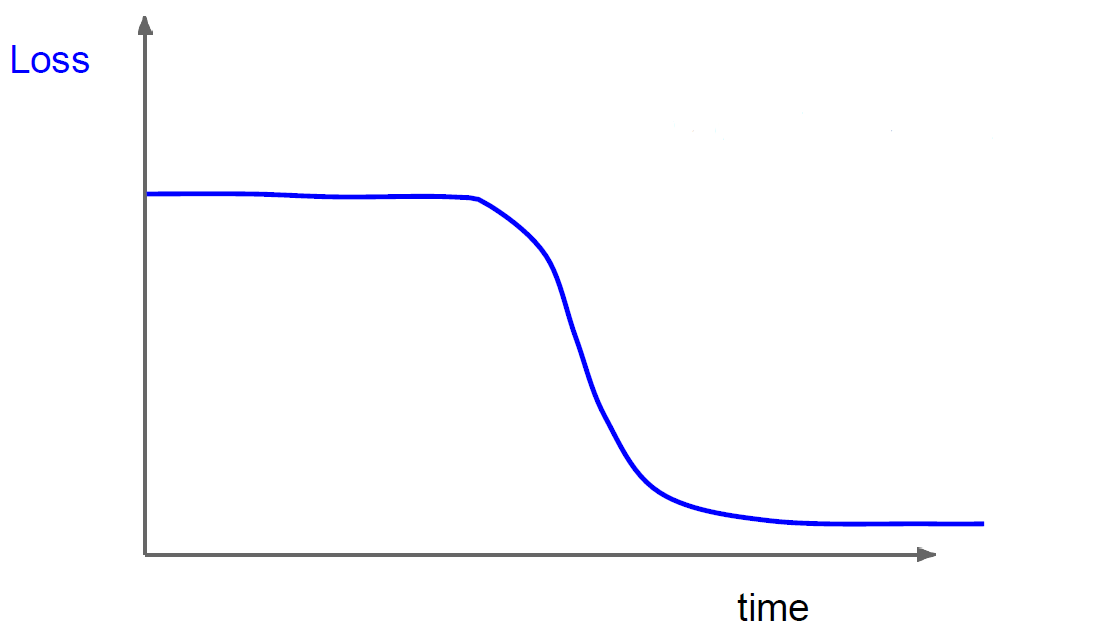
\includegraphics[width=0.9\linewidth]{images/tnn-loss-1}
        \caption[Loss drop]{Loss drop}
        \label{fig:tnn-loss-1}
    \end{figure}
\end{minipage}
\begin{minipage}{.3\linewidth}
    \begin{figure}[H]
        \centering
        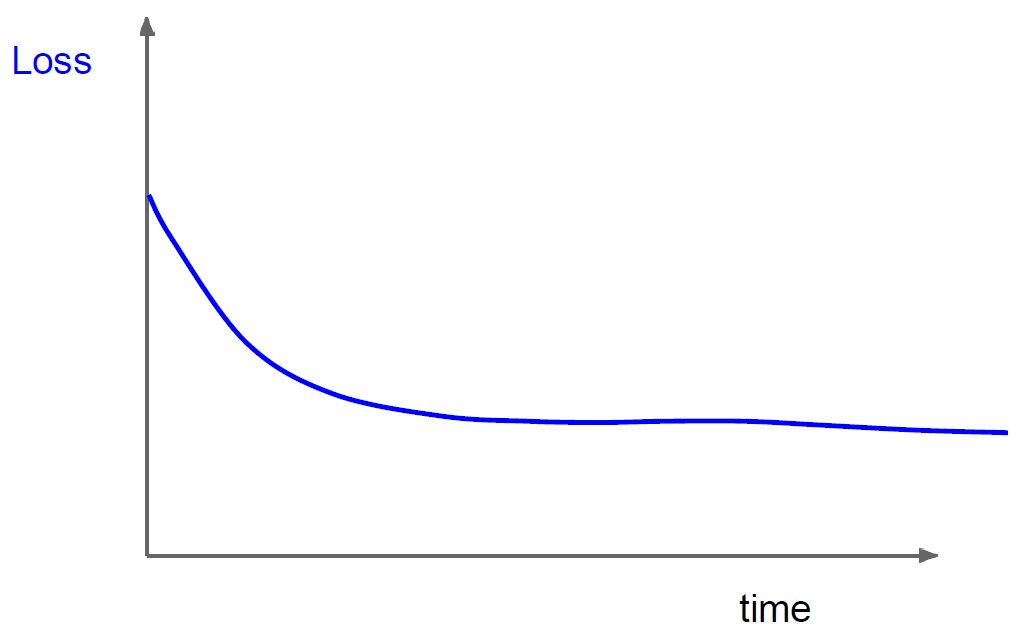
\includegraphics[width=0.9\linewidth]{images/tnn-loss-2}
        \caption[Loss plateaus]{Loss plateaus}
        \label{fig:tnn-loss-2}
    \end{figure}
\end{minipage}
\begin{minipage}{.3\linewidth}
    \begin{figure}[H]
        \centering
        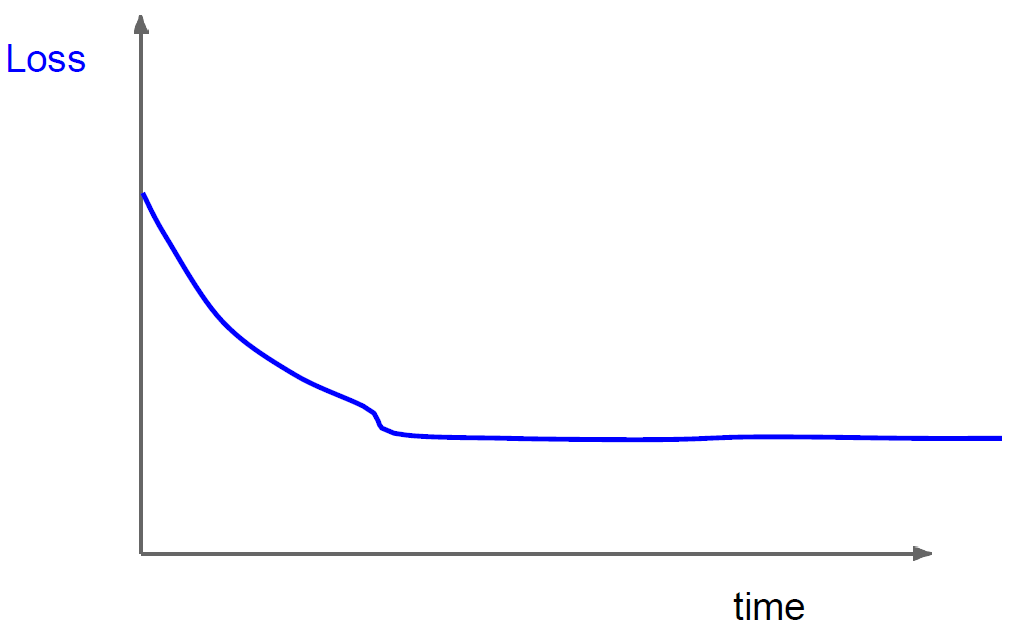
\includegraphics[width=0.9\linewidth]{images/tnn-loss-3}
        \caption[Learning rate step decay]{Learning rate step decay}
        \label{fig:tnn-loss-3}
    \end{figure}
\end{minipage}

\begin{minipage}{.3\linewidth}
    \begin{figure}[H]
        \centering
        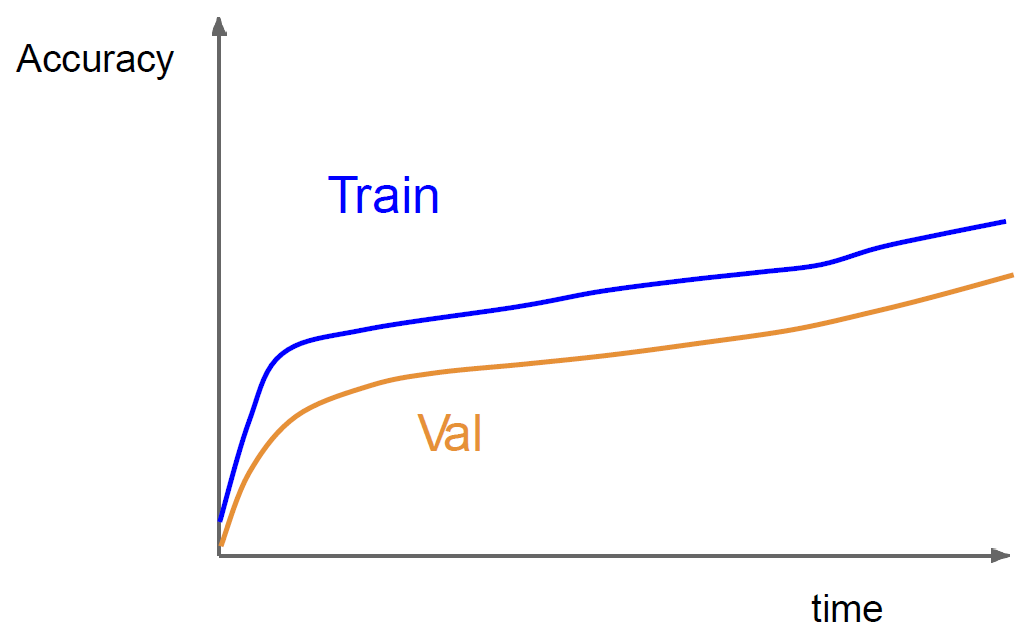
\includegraphics[width=0.9\linewidth]{images/tnn-acc-1}
        \caption[Accuracy still going up]{Accuracy still going up}
        \label{fig:tnn-acc-1}
    \end{figure}
\end{minipage}
\begin{minipage}{.3\linewidth}
    \begin{figure}[H]
        \centering
        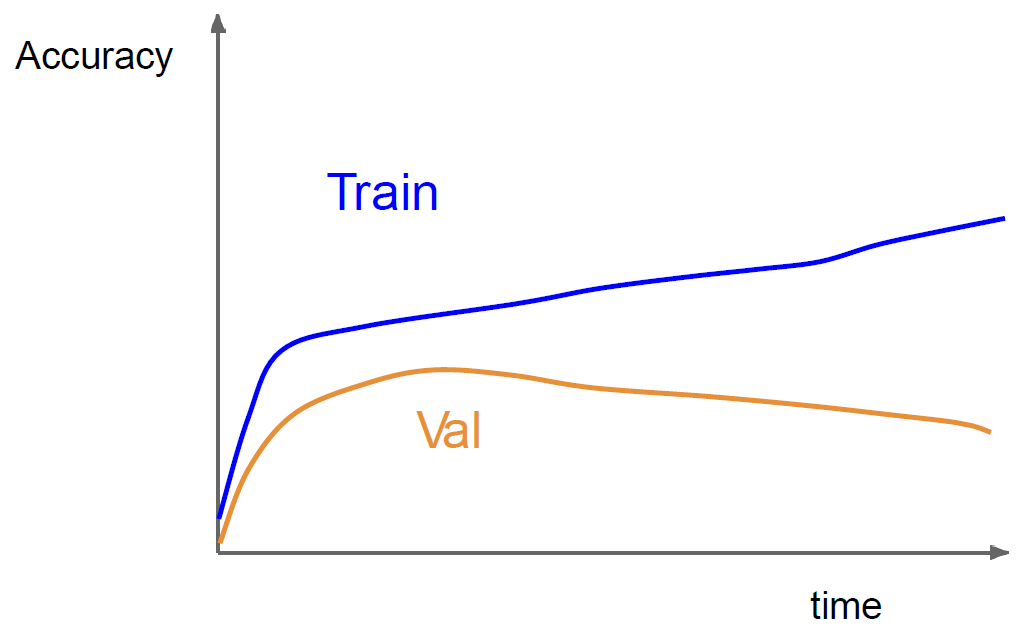
\includegraphics[width=0.9\linewidth]{images/tnn-acc-2}
        \caption[Huge train/val gap]{Huge train/val gap}
        \label{fig:tnn-acc-2}
    \end{figure}
\end{minipage}
\begin{minipage}{.3\linewidth}
    \begin{figure}[H]
        \centering
        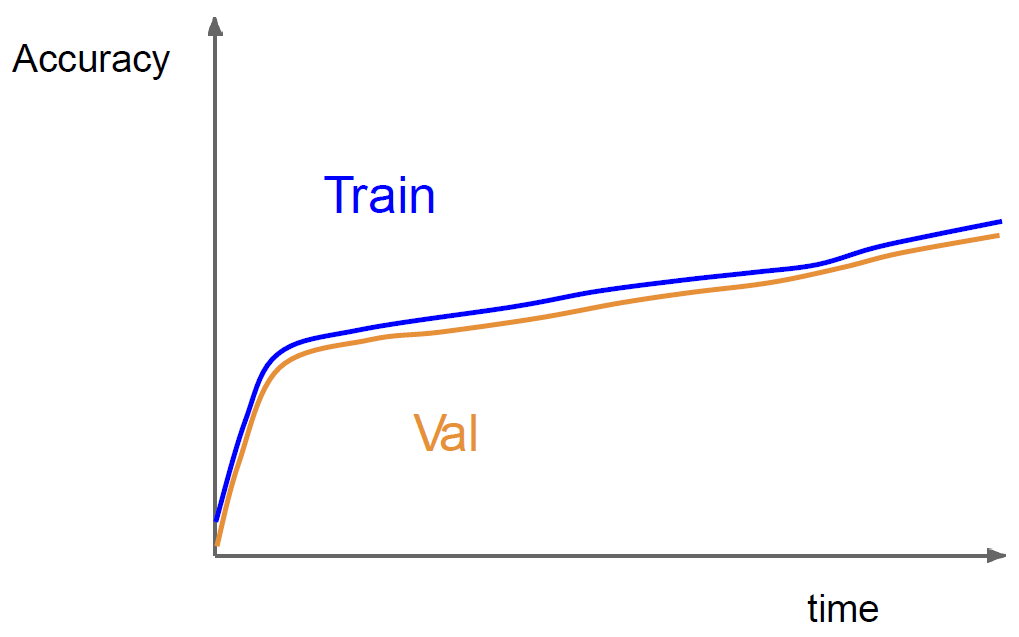
\includegraphics[width=0.9\linewidth]{images/tnn-acc-3}
        \caption[No train/val gap]{No train/val gap}
        \label{fig:tnn-acc-3}
    \end{figure}
\end{minipage}

Possible hyperparameters to tune are network architecture, learning rate and relative decay schedule, update type, regularization.

It is useful to track the ratio of weight updates/weight magnitudes: we want this to be somewhere around 0.001 or so.


\subsection{Transfer Learning}\label{sec:tnn-transfer}

The basic idea of \textit{transfer learning} is to train a big CNN model on a huge generic dataset, then freeze most of its layers and reuse the previous learned weights to train just the last layer(s) on the smaller task-specific dataset.

\begin{figure}[h!]
    \centering
    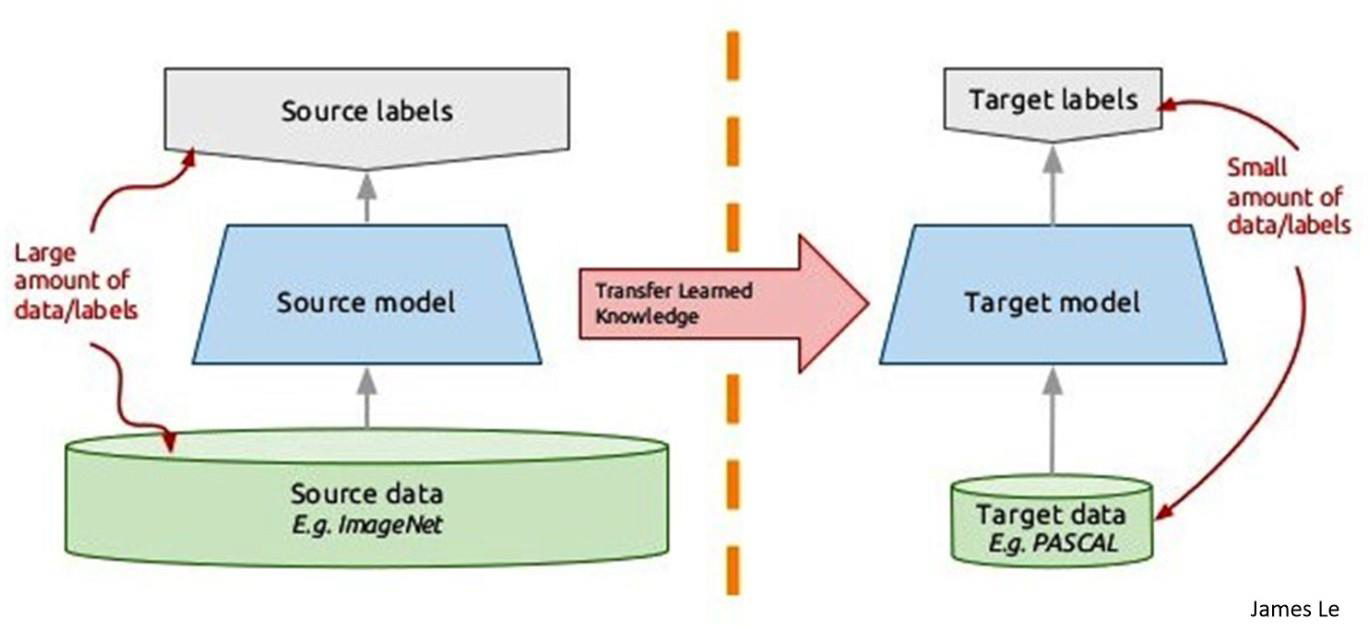
\includegraphics[width=0.7\linewidth]{images/transfer-learning}
    \caption[Transfer-learning]{Transfer-learning}
    \label{fig:transfer-learning}
\end{figure}

Depending on the situation, we need to use different approaches:
\begin{myitem}
    \item very little data and very similar datasets: use linear classifier on top layer;
    \item very little data but very different datasets: try linear classifier from different stages (but there is little to do in this case);
    \item quite a lot of data and very similar datasets: finetune a few layers;
    \item quite a lot of data and very different datasets: finetune a larger number of layers.
\end{myitem}

Always keep in mind that first layers are more generic, while last layers are more specific.

Transfer learning with CNNs is pervasive, but recent results show it might not always be necessary.
\begin{myitem}
    \item ImageNet pre training speeds up convergence early in training, but does not necessarily provide regularization or improve final target task accuracy;
    \item Sufficiently long training time can compensate for the lack of pre-training;
    \item Training from scratch may be superior to pre-training when the task is different;
    \item \textit{BatchNorm} is important for training from scratch but it is generally removed after pre-training.
\end{myitem}
